\documentclass{article}
\usepackage[dvipsnames]{xcolor}
\newcommand{\skipline}{\vskip 0.2in}

\usepackage[mast]{dennis}

\title{Cartesian Coordinates}
\author{Brian Zhang}
\date{GPV}

\begin{document}
\maketitle
\section{Theory}

Here are a couple of useful theorems.

\begin{theo}[Shoelace]
In a polygon with coordinates $(x_1,y_1),(x_2,y_2),\dots,(x_n,y_n)$, the area $\mathbf{A}$ is:
\begin{align*}
    \mathbf{A} &= \frac{1}{2}\left|\left(\sum_{i=1}^{n-1}x_iy_{i+1}\right)+ x_ny_1-\left(\sum_{i=1}^{n-1}x_{i+1}y_i\right)-x_1y_n\right|\\ 
    &=\frac{1}{2}\cdot |x_1y_2+x_2y_3+\cdots + x_{n-1}y_n+x_ny_1-x_2y_1-x_3y_2-\dots-x_ny_{n-1}-x_1y_n|.
\end{align*}
\end{theo}

\begin{theo}[Point to Line]
The distance between the point $(x_0,y_0)$ to the line $Ax+By+C=0$ can be written as 
\[\frac{|Ax_0+By_0+C|}{\sqrt{A^2+B^2}}.\]
\end{theo}

\begin{theo}[Coordinates of the Centroid]
In a triangle with coordinates $A=(x_a,y_a),B=(x_b,y_b),C=(x_c,y_c)$, the coordinates of the centroid is
\[\left(\frac{x_a+x_b+x_c}{3},\frac{y_a+y_b+y_c}{3}\right).\]
\end{theo}

\section{Heuristics}
\begin{itemize}
    \item Many people say that coordinate bashing is a ``no brain" technique, and is for when you don't know how to synthetic the geometry. This is false. When coordinate bashing, the most important step is your set up. This means what you define as the origin, and the equations of circles, lines, etc. Having the right setup will save you lots of time.
    \item Have a plan. Whenever I use coordinates on a problem, I plan out how I would calculate each point, and the method of calculating each point. This helps you get a sense of how long it will take you to solve the problem, and whether its worth it to just move onto another problem, or to try to look for a synthetic solution. 
    \item Know when to apply coordinates! Right angles, lots of lines, problems where you are given triangle side lengths are your friend. Some things that are harder to deal with are incenters, multiple circles, etc.
    \item Angle conditions are usually pretty hard to deal with, but if they can be reduced to the angle bisector theorem, cyclic quadrilaterals, or tangents, then it is much easier to deal with them. 
    \item When you have a nice central circle, its a good idea to set that circle at the origin, so the equation of the circle is easier to work with.
    \item For obvious reasons, knowledge of standard geometry theorems is also very helpful. If you can use synthetic techniques to help you simplify the problem, then coordinate bashing can be much less computationally heavy and much faster. 
    \item When given a triangle with three side lengths, then you can use Heron's to calculate the area, and then calculate the altitude of one of the sides, so you can place the triangle onto the coordinate plane. 
\end{itemize}

\section{Examples}

\begin{exam}
Let $ABC$ be a triangle with $AB=13$, $BC=14$, $AC=15$. Let $H,I,M$ be the orthocenter of $\Delta ABC$, incenter of $\Delta ABC$, and midpoint of $BC$ respectively. What is the area of $\Delta HIM$?
\end{exam}

\begin{walk}

\begin{enumerate}
    \item As usual, we want to set $A=(0,a)$, $B=(b,0)$, $C=(c,0)$. Find the values of $a,b,c$. 
    \item For $H$, we can drop an altitude from $B$ to $CA$, and find the intersection of that with the $A$ altitude.
    
    We could calculate the location of $I$ by creating two angle bisectors, and using angle bisector theorem, but there is a better way. 

    \item Instead, we can calculate the inradius, and note that the $y$-coordinate of the incenter is equal to the inradius.
    \item For the $x$-coordinate, we can just use the formulas for distances between the vertices of triangles and the incircle touch points. Alternatively, you could calculate the $A$-angle bisector with angle bisector theorem and intersect that with $y=r$, where $r$ is the inradius.
    \item Finish using a good area formula. 
\end{enumerate}

\end{walk}

\begin{exam}[AMC 10A 2020/20]
Quadrilateral $ABCD$ satisfies $\angle ABC = \angle ACD = 90^{\circ}, AC=20,$ and $CD=30.$ Diagonals $\overline{AC}$ and $\overline{BD}$ intersect at point $E,$ and $AE=5.$ What is the area of quadrilateral $ABCD?$
\end{exam}

\begin{walk}

\begin{enumerate}
    \item We could set the origin to be $C$, as we have $CD$ and $AC$, but there actually is a better point to use. (If you can't figure out where this is, then think about how we know $AC$, and $\angle ABC=90^{\circ}$.)
    
    You should have set the origin to be the midpoint of segment $AC$. We are motivated to do this because this allows us to draw a circle $\omega$ centered at the origin that passes through $A$ and $C$, and note that $B$ also passes through the circle.
    
    \item Find the equation to the circle $\omega$, and calculate $B$ by defining it as the second intersection of $\omega$ with $DE$. 
    \item You should get a quadratic. Elimnate the "wrong" solution.
    \item Finish. 
\end{enumerate}

\end{walk}

Here is an instructional problem demonstrating point to line that some of you may be slighlty familiar with. 
\begin{exam}[AIME I 2021/9]
Let $ABCD$ be an isosceles trapezoid with $AD=BC$ and $AB<CD.$ Suppose that the distances from $A$ to the lines $BC,CD,$ and $BD$ are $15,18,$ and $10,$ respectively. Let $K$ be the area of $ABCD.$ Find $\sqrt2 \cdot K.$
\end{exam}

\begin{walk}

\begin{enumerate}
    \item Note how we have a bunch of distances from a point to several lines, with the point being on one of 2 parallel lines. What are we motivated to use?
    \item Find a nice point that we can set as the origin, so that the coordinates of $A,B,C,D$ are all relatively clean.
    
    What I found to be the cleanest was to set the foot of the altitude from $A$ to $CD$ to be the origin, although some other solutions used different origins. 
    
    \item Use point to line from $A$ to $BC$ and $BD$ to get two equations.
    
    You should have gotten the quadratics 
    \begin{align*}
        \sqrt{324+(b+d)^2}&=\frac{9}{5}b\\
        \sqrt{324+d^2}&=\frac{6}{5}b
    \end{align*}
    or some equivalent expression. This may be slightly different based on how you chose your variables and the origin. 
    \item Solve for $b$ and $d$, by squaring and subtracting. 
    \item Finish. 
\end{enumerate}

\end{walk}

\pagebreak
\section{Problems}

\minpt{34}

\psetquote{Let's flippin' get this coordinate bash on with.}{Neil Shah}

\prob{2}{MATHCOUNTS 2008}{In triangle $\Delta ABC$ with $\angle C = 90$, points $E$ and $F$ are on sides $CA$ and $CB$, respectively with $CE=2$ and $CF=3$. Given that $D$ is the intersection of lines $AF$ and $BE$, and the area of $\Delta ABD$ can be written as $\frac{m}{n}$ with $\gcd(m,n)=1$, then find the value of $m+n$.}

% nats team 2008/10

\prob{3}{AMC 10B 2004/18}{In the right triangle $\triangle ACE$, we are given that  $AC=12$, $CE=16$, and $EA=20$. Let the points $B$, $D$, and $F$ be located on $AC$, $CE$, and $EA$, respectively, so that $AB=3$, $CD=4$, and $EF=5$. If the value of $\frac{[\triangle DBF]}{[\triangle ACE]}$ is equal to $\frac{m}{n}$, where $\gcd(m,n)=1$, then find the value of $m$ + $n$.}

\prob{3}{AMC 10A 2018/23}{Farmer Kevin has a field of corn in the shape of a right triangle. The right triangle's legs have lengths 3 and 4 units. In the corner where those sides meet at a right angle, he leaves a small unplanted square $S$ so that from the air it looks like the right angle symbol. The rest of the field is planted. The shortest distance from $S$ to the hypotenuse is 2 units. Given that the fraction of the field that is planted can be written as $\frac{m}{n}$ where $\gcd(m,n)=1$, then find the value of $m+n$.
\begin{center}
    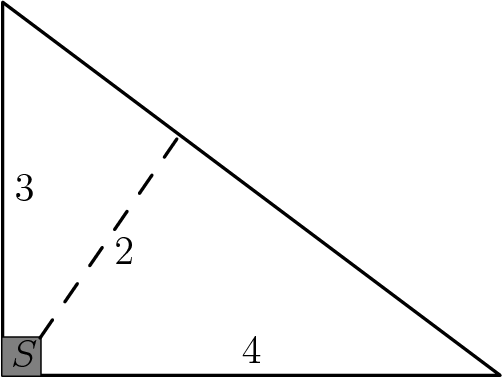
\includegraphics[width=0.4\textwidth]{pythagoras.png}
\end{center}}

\prob{3}{AMC 10A 2016/19}{In rectangle $ABCD$, $AB=6$ and $BC=3$. Point $E$ between $B$ and $C$, and point $F$ between $E$ and $C$ are such that $BE=EF=FC$. Segments $\overline{AE}$ and $\overline{AF}$ intersect $\overline{BD}$ at $P$ and $Q$, respectively. The ratio $BP:PQ:QD$ can be written as $r:s:t$, where the greatest common factor of $r,s$ and $t$ is $1$. What is $r+s+t$?}

\prob{3}{AMC 10A 2014/16}{n rectangle $ABCD$, $AB=1$, $BC=2$, and points $E$, $F$, and $G$ are midpoints of $\overline{BC}$, $\overline{CD}$, and $\overline{AD}$, respectively. Point $H$ is the midpoint of $\overline{GE}$. What is the area of the shaded region?
\begin{center}
    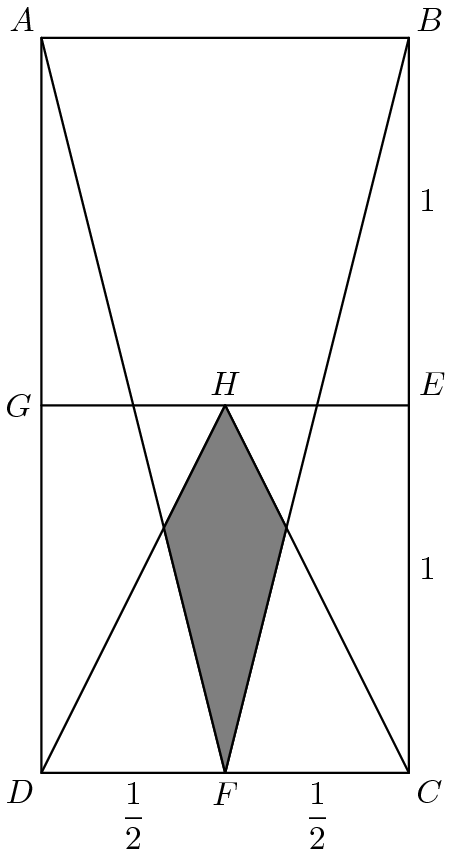
\includegraphics[width=0.3\textwidth]{amc-2014.png}
\end{center}
}

\prob{4}{CIME I 2021/5}{In rectangle $ABCD$, suppose $AD = 20$ and $AB = 21$. The circle centered at $A$ passing through $D$ intersects the circle centered at $C$ passing through $D$ at a point $P \neq D$. Then the length $BP$ can be written in the form $\frac{p}{q}$, where $p$ and $q$ are relatively prime positive integers. Find $p + q$.}

\prob{4}{AIME I 2015/4}{Point $B$ lies on line segment $\overline{AC}$ with $AB=16$ and $BC=4$. Points $D$ and $E$ lie on the same side of line $AC$ forming equilateral triangles $\triangle ABD$ and $\triangle BCE$. Let $M$ be the midpoint of $\overline{AE}$, and $N$ be the midpoint of $\overline{CD}$. The area of $\triangle BMN$ is $x$. Find $x^2$.}

\prob{6}{AIME II 2018/9}{Octagon $ABCDEFGH$ with side lengths $AB = CD = EF = GH = 10$ and $BC=  DE = FG = HA = 11$ is formed by removing four $6-8-10$ triangles from the corners of a $23\times 27$ rectangle with side $\overline{AH}$ on a short side of the rectangle, as shown. Let $J$ be the midpoint of $\overline{HA}$, and partition the octagon into $7$ triangles by drawing segments $\overline{JB}$, $\overline{JC}$, $\overline{JD}$, $\overline{JE}$, $\overline{JF}$, and $\overline{JG}$. Find the area of the convex polygon whose vertices are the centroids of these $7$ triangles.
\begin{center}
    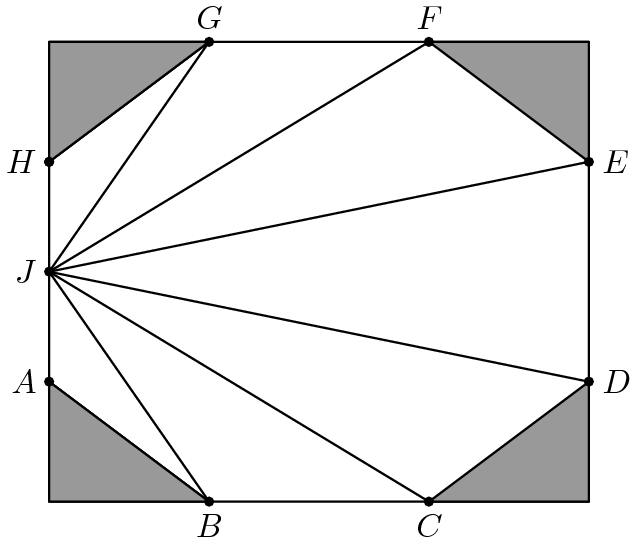
\includegraphics[width = 0.4\textwidth]{problem_4.png}
\end{center}}

\prob{6}{AIME II 2017/10}{Rectangle $ABCD$ has side lengths $AB=84$ and $AD=42$. Point $M$ is the midpoint of $\overline{AD}$, point $N$ is the trisection point of $\overline{AB}$ closer to $A$, and point $O$ is the intersection of $\overline{CM}$ and $\overline{DN}$. Point $P$ lies on the quadrilateral $BCON$, and $\overline{BP}$ bisects the area of $BCON$. Find the area of $\triangle{CDP}$.}

\prob{6}{AIME II 2003/11}{Triangle $ABC$ is a right triangle with $AC=7,$ $BC=24,$ and right angle at $C.$ Point $M$ is the midpoint of $AB,$ and $D$ is on the same side of line $AB$ as $C$ so that $AD=BD=15.$ Given that the area of triangle $CDM$ may be expressed as $\frac{m\sqrt{n}}{p},$ where $m,$ $n,$ and $p$ are positive integers, $m$ and $p$ are relatively prime, and $n$ is not divisible by the square of any prime, find $m+n+p.$}

\prob{9}{CIME II 2021/12}{Let $ABC$ be a triangle with $AB = 5, BC = 6, CA = 7$. Let $O$ be the circumcenter of $\triangle ABC$ and let $P$ be a point such that $AB \perp BP$ and $AC \perp AP$. If lines $OP$ and $BC$ intersect at $T$, then find $BT$.}

\prob{9}{AIME I 2020/13}{Point $D$ lies on side $BC$ of $\triangle ABC$ so that $\overline{AD}$ bisects $\angle BAC$. The perpendicular bisector of $\overline{AD}$ intersects the bisectors of $\angle ABC$ and $\angle ACB$ in points $E$ and $F$, respectively. Given that $AB=4$, $BC=5$, $CA=6$, the area of $\triangle AEF$ can be written as $\tfrac{m\sqrt n}p$, where $m$ and $p$ are relatively prime positive integers, and $n$ is a positive integer not divisible by the square of any prime. Find $m+n+p$.}

\pagebreak

\appendix

\section{Solutions to Examples}
\subsection{Unsourced}
We set $A=(0,12),B=(-5,0),C=(9,0)$. Its easy to see that $M=(2,0)$. Now, basic computation gives us the inradius $r=4$. If we let $D$ be the $BC$ touchpoint of the incircle, then it isn't hard to see that $BD=5$, so $I=(1,5)$. Dropping altitudes gives $H=(0,\frac{15}{4})$, so we can use shoelace to get the answer of $\boxed{\frac{17}{8}}$.

\subsection{AMC 10A 2020/20}
\begin{center}
    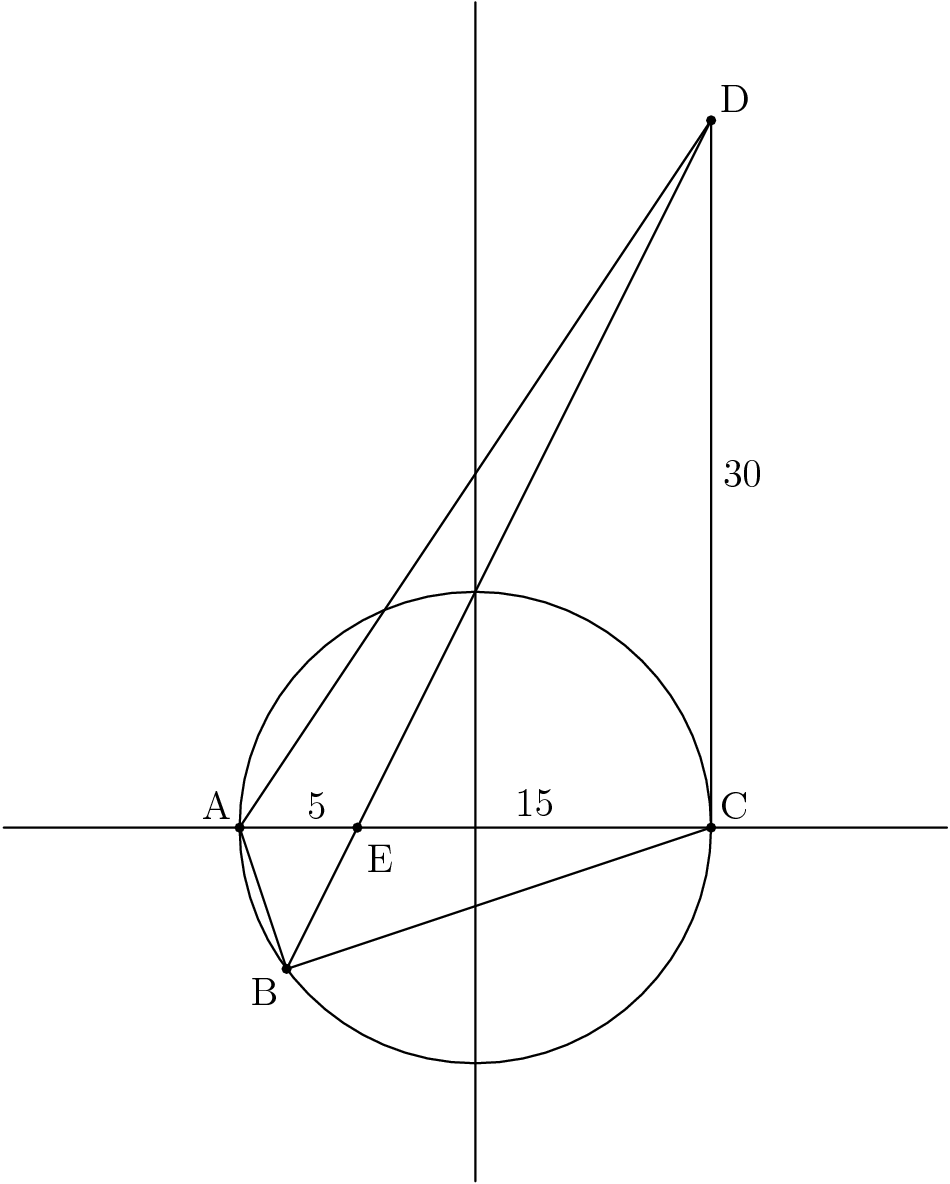
\includegraphics[width = 0.5\textwidth]{amc2020.png}\\
    \textit{Diagram from AoPS Wiki.}
\end{center}
We set the origin to be the midpoint of $AC$. Now, construct $(ABC)$, and note that the equation of $(ABC)$ is $x^2+y^2=100$. We have the coordinates are
\begin{align*}
    A&=(-10,0)\\
    C&=(10,0)\\
    D&=(10,30)\\
    E&=(-5,0)
\end{align*}
It remains to calculate $B$. Now, note that $B$ is simply the intersection of $x^2+y^2=100$ and line $DE$. But line $DE$ can be easily calculated to be $y=-2(x+5)$ from point slope formula. It remains to solve 
\begin{align*}
    x^2+(-2(x+5))^2&=100\\
    \implies 5x^2+40x&=0\\
    \implies x&=-8,0
\end{align*}
Obviously, $x=0$ is the first intersection of $DE$ with $(ABC)$, so we can toss that out. Then, plugging $x=-4$ back in we get $y=-6$. Finally, we finish with shoelace on $ABCD$, and get an answer of $\boxed{360}$.

\subsection{AIME I 2021/9}
Instead of high IQ similar triangle spam, we use the method of coordinate bashing. We do this by setting the origin to be the foot from $A$ to $CD$, and noting that we can use point to line formula and isosceles trapezoid properties to get the locations of the points $B,C,D$. 

We let $X$, $Y$, $Z$ be the feet of the altitudes from $A$ to $CD$, $DB$, and $BC$, respectively.  

Now, setting $X$ as the origin, we can set
\begin{align*}
    A&=(0,18)\\
    B&=(b,18)\\
    C&=(b+d,0)\\
    D&=(-d,0)\\
    X&=(0,0)
\end{align*}
We want to use point to line, so we need the equations of $BC$ and $BD$. It's pretty easy to get
\begin{align*}
    BD&:y=\frac{18}{b+d}(x+d)\\
    BC&:y=\frac{18}{-d}(x-b-d)
\end{align*}
Now, point to line on $A$ to $BD$ and $BC$ gives 
\begin{align*}
    10&=\frac{-18(b+d)+18d}{\sqrt{324+(b+d)^2}}\\
    15&=\frac{18d+18(-b-d)}{\sqrt{18^2+d^2}}
    \intertext{respectively. Now, rearranging, we get}
    \sqrt{324+(b+d)^2}&=\frac{9}{5}b\\
    \sqrt{324+d^2}&=\frac{6}{5}b
    \intertext{This is equivalent to}
    324+b^2+2bd+d^2&=\frac{81}{25}b^2\\
    324+d^2&=\frac{36}{25}b^2
\end{align*}
Upon subtracting the two equations, we get $d=\frac{2}{5}b$. Now plugging this back into $324+d^2=\frac{36}{25}b^2$, we get 
\begin{align*}
    324+\frac{4}{25}b^2&=36b^2\\
    \implies 324=\frac{32}{25}b^2\\
    \implies b=\frac{45\sqrt{2}}{4}\\
    \implies d=\frac{9\sqrt{2}}{2}
\end{align*}
From here it is not hard to get the answer of $\boxed{567}$.

\skipline
\noindent
\textbf{Remark:} On contest, I calculated the area of the trapezoid to be $\frac{1}{2}\cdot(b+d)\cdot b\cdot18\implies 486$. Oops.

\end{document}
